\section{Introduction}
\label{sec:intro}

\lightlipsum[1]

\begin{figure} [h]
	\begin{center}
	% Replace with topological map
	\begin{subfigure}[b]{0.45\textwidth}
		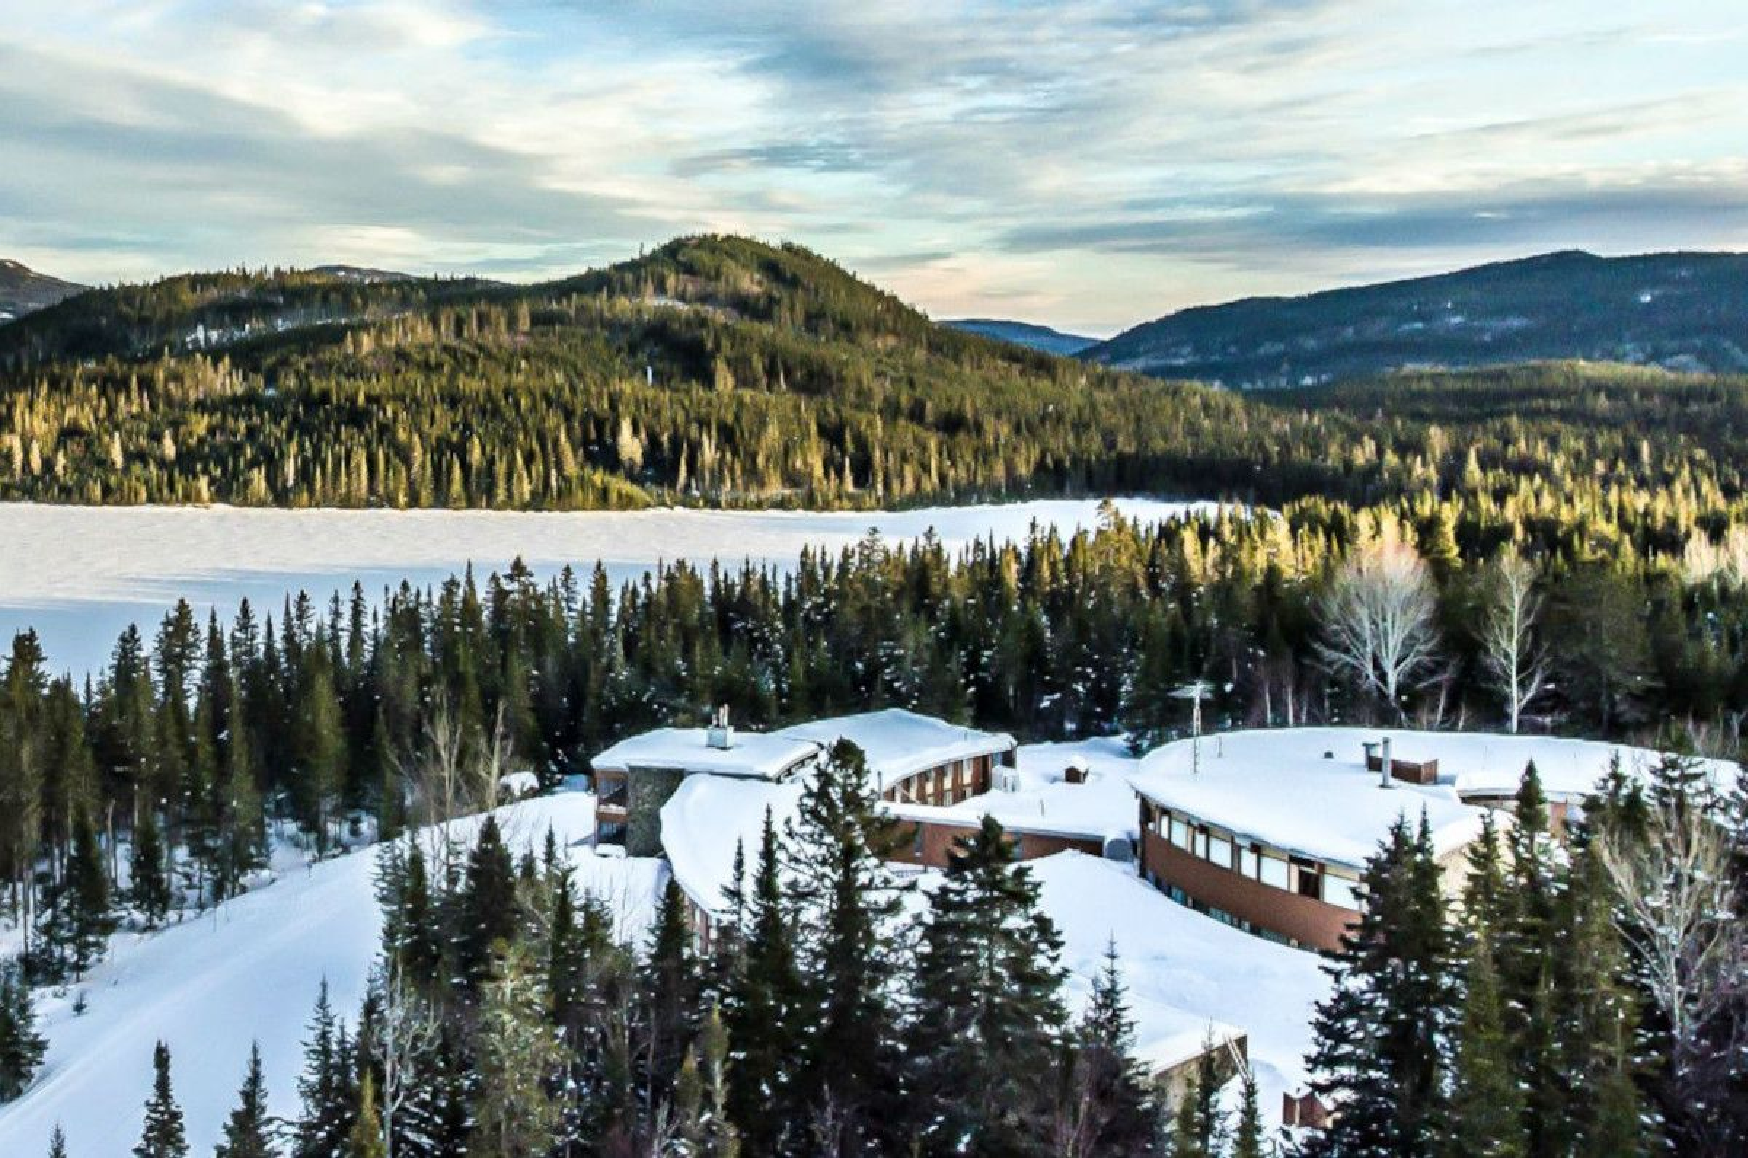
\includegraphics[width=\linewidth]{figs/foret-montmorency.pdf}
		%\caption{A view from above the \textit{Montmorency} boreal forest, which served the purpose of test area for this work.}
		\label{fig:view_above}
	\end{subfigure}%
	~~
	% replace with aerial?
	\begin{subfigure} [b] {0.45\textwidth}
		\includegraphics[width=\linewidth]{figs/warthog_laverdiere.pdf}
		%\caption{Shot of our system parked in front of the \laverdiere~cottage.}
		\label{fig:front_fig}
	\end{subfigure}
	\end{center}
	\caption{Our \ac{LTR} framework was designed to be used in subarctic environments.
	The \textit{Montmorency} boreal forest is an ideal example of such areas.
	The image on the right shows our \ac{UGV} parked at the end of one of our defined paths.
	Image credit : \foretmo.}
	\label{fig:intro}
\end{figure}

\lightlipsum[1]
\lightlipsum[1]
\lightlipsum[1]

% Discuss lifelong learning